\section{Context Free Grammars}

\begin{multicols*}{2}
\setlength{\columnsep}{1.5cm}
\setlength{\columnseprule}{0.2pt}

\begin{itemize}
  \item \textbf{Language Recognizer:} A device that accepts valid strings. For example, finite automata are language recognizer.
  \item \textbf{Language Generator:} A device that generates valid strings.
\end{itemize}

We shall study certain types of formal language generators. Such a device begins, when given some sort of ``start'' signal, to construct a string. Its operation is \textit{not completely determined from the beginning but is nevertheless limited by a set of rules}. Eventually this process halts, and the device outputs a completed string. \textit{The language defined by the device is the set of all strings that it can produce.}

Neither a recognizer nor a generator for the English language is at all easy
to produce. Nevertheless, the idea of a language generator has some explanatory force in attempts to discuss human language. More important for us, however, is \textit{the theory of generators of formal}, ``artificial'' languages, such as the regular languages and the important class of ``context-free'' languages will be introduced.

This theory will neatly \textit{complement the study of automata}, which recognize languages, and is also of practical value in the specification and analysis of computer languages.\\

Regular expressions can be viewed as language generators. 

\noindent For example, consider the regular expression $a(a^* \cup b^*)b$.A verbal description of how to generate a string in accordance with this expression would be the following
\begin{itemize}
  \item First output an $a$. Then do one of the following two things:
  \item Either output a number of $a$'s or output a number of $b$'s.
  \item Finally output a $b$
\end{itemize}
The language associated with this language generator -that is, the set of
all strings that can be produced by the process just described- is, of course, exactly the regular language defined in the way described earlier by the regular expression $a(a^* \cup b^*)b$. 

We will study certain more complex sorts of language generators, called \textbf{context-free grammars}, which are based on a more complete understanding of the structure of the strings belonging to the language.


To take again the example of the language generated by $a(a^* \cup b^*)b$. If we let $S$ be a new symbol interpreted as ``\textit{a string in the language}'', and $M$ be a symbol standing for ``\textit{middle part}'', then we can express this observation by writing
\begin{equation*}
  S \to aMb
\end{equation*}
where $\to$ is read ``\textit{can be}''. We call such an expression a \textbf{rule}. What can $M$, the middle part, be? The answer is: either a string of $a$'s or a string of $b$'s.

\vspace*{\fill}
\columnbreak

\noindent We express this by adding the rules
\begin{align*}
  M \to A \textnormal{    and    } M \to B
\end{align*}
where $A$ and $B$ are new symbols that stand for strings of $a$'s and $b$'s, respectively. Now, what is a string of $a$'s? It can be the empty string
\begin{equation*}
  A \to e
\end{equation*}
or it may consist of a leading a followed by a string of $a$'s:
\begin{equation*}
  A \to aA
\end{equation*}
Similarly, for $B$:
\begin{equation*}
  B \to e \textnormal{    and    } B \to bB
\end{equation*}
The language denoted by the regular expression $a(a^* \cup b^*)b$ can then be defined alternatively by the following language generator.
\begin{quote}
  Start with the string consisting of the single symbol $S$. Find a symbol in the current string that appears to the left of $\to$ in one of the rules above. Replace an occurrence of this symbol with the string that appears to the right of $\to$ in the same rule. Repeat this process until no such symbol can be found.
\end{quote}

For example, to generate the string $aaab$ we start with $S$, as specified; we then replace $S$ by $aMb$ according to the first rule, $S \to aMb$. To $aMb$ we apply the rule $M \to A$ and obtain $aAb$. We then twice apply the rule $A \to aA$ to get the string $aaaAb$. Finally, we apply the rule $A \to e$. In the resulting string, $aaab$, we cannot identify any symbol that appears to the left of $\to$ in some rule. Thus the operation of our language generator has ended, and $aaab$ was produced, as promised.

A \textbf{context-free grammar} is a language generator that operates like the one above, with some such set of rules. Let us pause to explain at this point \textit{why such a language generator is called context-free}. Consider the string $aaAb$, which was an intermediate stage in the generation of $aaab$. It is natural to call the strings $aa$ and $b$ that surround the symbol $A$ the \textbf{context of $A$} in this particular
string. Now, the rule $A \to aA$ says that we can replace $A$ by the string $aA$ no matter what the surrounding strings are; in other words, \textit{independently of the context of $A$}.

In a context-free grammar, some symbols appear to the left of $\to$ in rules -$S$, $M$, $A$, and $B$ in our example- and some -$a$ and $b$- do not. Symbols of the latter kind are called \textbf{terminals}, since the production of a string consisting solely of such symbols signals the termination of the generation process. All these ideas can be stated formally.
\end{multicols*}

\begin{definition}{}
  A \textbf{context-free grammar} $G$ is a quadruple $(V, \Sigma, R, S)$ where
  \begin{itemize}
    \item $V$ is an alphabet
    \item $\Sigma$ (the set of \textbf{terminals}) is a subset of $V$
    \item $R$ (the set of \textbf{rules}) is a finite subset of $(V - \Sigma) \times V^*$
    \item $S$ (the \textbf{start symbol}) is an element of $V - \Sigma$
  \end{itemize}
  The members of $V - \Sigma$ are called \textbf{nonterminals}. For any $A \in V - \Sigma$ and $u \in V^*$, we write $A \rightarrow_G u$ whenever $(A, u) \in R$. For any strings $u, v \in V^*$, we write $u \Rightarrow_G v$ if and only if there are strings $x, y \in V^*$ and $A \in V - \Sigma$ such that $u = xAy$, $v = xv'y$, and $A \rightarrow_G v'$. The relation $\Rightarrow_G^*$ is the \textit{reflexive}, \textit{transitive closure} of $\Rightarrow_G$. Finally, $L(G)$, the \textbf{language generated} by $G$, is $\left\{ w \in \Sigma^* : S \Rightarrow_G^* w \right\}$; we also say that $G$ \textbf{generates} each string in $L(G)$. A language $L$ is said to be a \textbf{context-free language} if $L = L(G)$ for some context-free grammar $G$.
\end{definition}

\noindent When the grammar to which we refer is obvious, we write $A \to w$ and $u \Rightarrow v$ instead of $A \to_G w$ and $u \Rightarrow_G v$.

We call any sequence of the form
\begin{equation*}
  w_0 \Rightarrow_G w_1 \Rightarrow_G \cdots \Rightarrow_G w_n
\end{equation*}
a \textbf{derivation} in $G$ of $w_n$ from $w_0$. Here $w_o, \cdots, w_n$ may be any strings in $V^*$, and $n$, the \textbf{length} of the derivation, may be any natural number, including zero. We also say that the derivation has $n$ \textbf{steps}. 

\begin{example_break}{}
  Consider the context-free grammar $G = (V, \Sigma, R, S)$, where
  \begin{itemize}
    \item $V = \{ S, a, b \}$
    \item $\Sigma = \{ a, b \}$
    \item $R$ consists of the rules $S \to aSb$ and $S \to e$.
  \end{itemize}
  A possible derivation is
  \begin{equation*}
    S \Rightarrow aSb \Rightarrow aaSbb \Rightarrow aabb.
  \end{equation*}
  Here the first two steps used the rule $S \to aSb$, and the last used the rule $S \to e$. In fact, it is not hard to see that $L(G) = \{ a^nb^n\ |\ n \geq 2 \}$. \textit{Hence some context-free languages are not regular, but all regular languages are context-free.}
\end{example_break}

\begin{example_break}{}
  Let $G$ be the grammar $(W, \Sigma, R, S)$, where
  \begin{align*}
    W = \{& S, A, N, V, P \} \cup \Sigma\\
    \Sigma = \{& \textnormal{Jim, big, green, cheese, ate} \}\\
    R = \{& P \to N,\\
          & P \to AP,\\
          & S \to PVP,\\
          & A \to \textnormal{big},\\
          & A \to \textnormal{green},\\
          & N \to \textnormal{cheese},\\
          & N \to \textnormal{Jim},\\
          & V \to \textnormal{ate} \}
  \end{align*}
  Here $G$ is designed to be a grammar for a part of English; $S$ stands for \textit{sentence}, $A$ for \textit{adjective}, $N$ for \textit{noun}, $V$ for \textit{verb}, and $P$ for \textit{phrase}. The following are some strings in $L(G)$.
  \begin{itemize}
    \item Jim ate cheese
    \item big Jim ate green cheese
    \item big cheese ate Jim
  \end{itemize}
  Unfortunately, the following are also strings in $L(G)$:
  \begin{itemize}
    \item big cheese ate green green big green big cheese
    \item green Jim ate green big Jim     
  \end{itemize}
\end{example_break}

\noindent \textbf{\textit{Note:}} \textit{Example 3.1.3, 3.1.4 and 3.1.5 should be read from book.}

\begin{formula}{}
  \begin{itemize}
    \item $u \Rightarrow v$: $u$ \textbf{\textit{directly yields}} $v$; $A \rightarrow w$: \textbf{\textit{(production) rule}}.
    \item $V$, alphabet, can include symbols such as start symbol, $S$, or $A$.
    \item (From example 3.1.4) The same string may have several derivations in a context-free grammar. Two derivations in this grammar are
    \begin{align*}
      &S \Rightarrow SS \Rightarrow S(S) \Rightarrow S((S)) \Rightarrow S(()) \Rightarrow ()(()) &\textnormal{ and } && S \Rightarrow SS \Rightarrow (S)S \Rightarrow ()S \Rightarrow ()(S) \Rightarrow ()(())
    \end{align*}
    \item Some context-free languages are not regular. However, all regular languages are context-free.
    \item Context-free languages are precisely the languages accepted by certain language acceptors called \textit{\textbf{pushdown automata}}.
  \end{itemize}
\end{formula}

\begin{figure}[h]
  \centering
  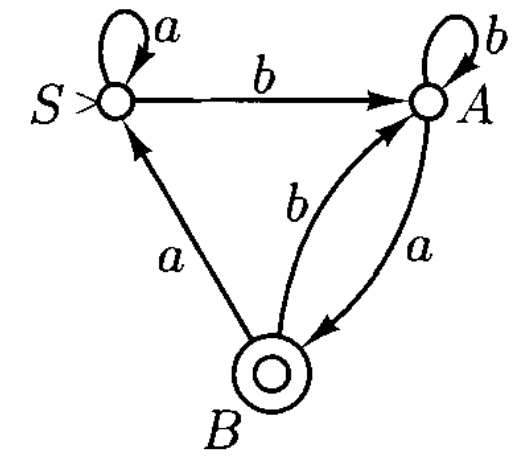
\includegraphics[width=.2\textwidth]{img/fig3-1.png}
  \caption{}
\end{figure}

\begin{proof}
  We can prove the statement ``\textit{all regular languages are context-free}'' by a \textit{\textbf{direct construction}}. Consider the regular language accepted by the deterministic finite automaton $M = (K, \Sigma, \delta, s, F)$. The same language is generated by the grammar $G(M) = (V, \Sigma, R, S)$, where $V = K \cup \Sigma$, $S = s$, and $R$ consists of these rules:
  \begin{equation*}
    R = \left\{ q \to ap\ |\ \delta(q, a) = p \right\} \cup \left\{ q \to e\ |\ q \in F \right\}
  \end{equation*}
  That is, the nonterminals are the states of the automaton; as for rules, for each transition from $q$ to $p$ on input $a$ we have in $R$ the rule $q \to p$. For example, for the automaton in Figure 1 we would construct this grammar:
  \begin{equation*}
    S \to aS,\ S \to bA,\ A \to aB,\ A \to bA,\ B \to aS,\ B \to bA,\ B \to e.
  \end{equation*}
\end{proof}
